\chapter{\;\;\;\;Program Verification}
\label{sec:program}

\todo{revise}
In \Cref{sec:overview-verification} we presented how to achieve compositional compiler correctness
%% ---namely adequacy, horizontal compositionality, and vertical compositionality---
in our framework.  In this section we present what our framework additionally offers about compiler and
program verification: verifying more advanced compiler optimizations with module-local
invariants (\Cref{sec:overview-modulelocal:compiler}) and verifying program modules against their
mathematical specification modules (\Cref{sec:overview-modulelocal:program} and \Cref{sec:overview-modulelocal:utod}).
\revision{To the best of our knowledge, our framework is the
first, in the context of \cc{}, that is capable of verifying
the \emph{mutually recursive} example presented in \Cref{sec:overview-modulelocal:program}.}






\subsection{Verification against Specification Modules}
\label{sec:overview-modulelocal:program}

\begin{figure}[t]
\makebox[\linewidth]{\makebox[1.1\linewidth]{
\begin{minipage}{1.1\linewidth}
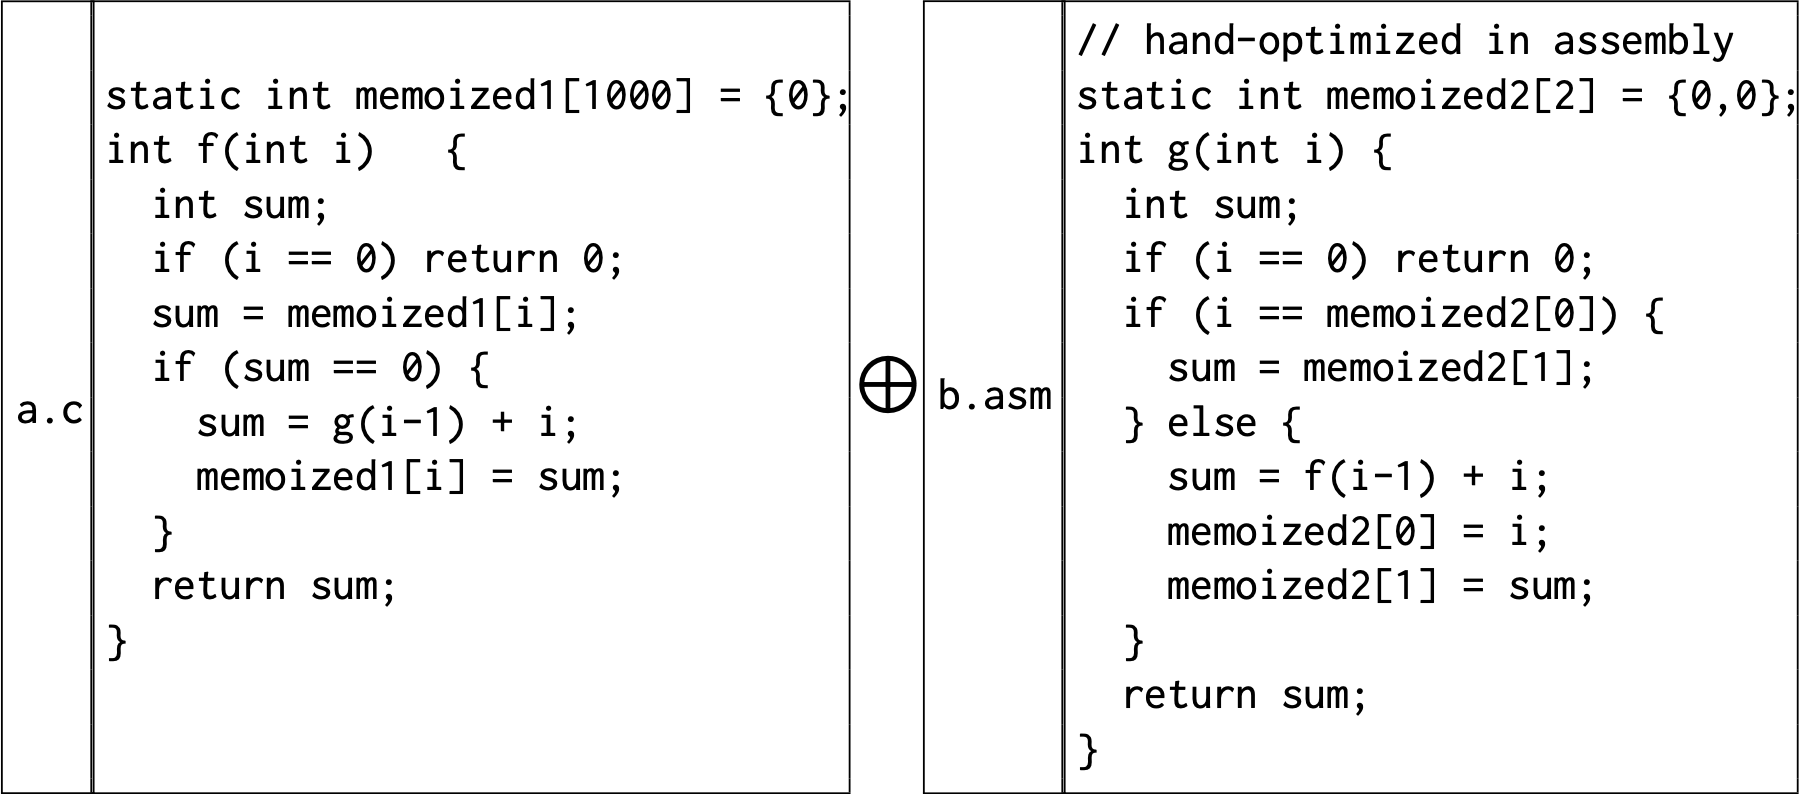
\includegraphics[width=1\linewidth]{images/mutsum1.png}
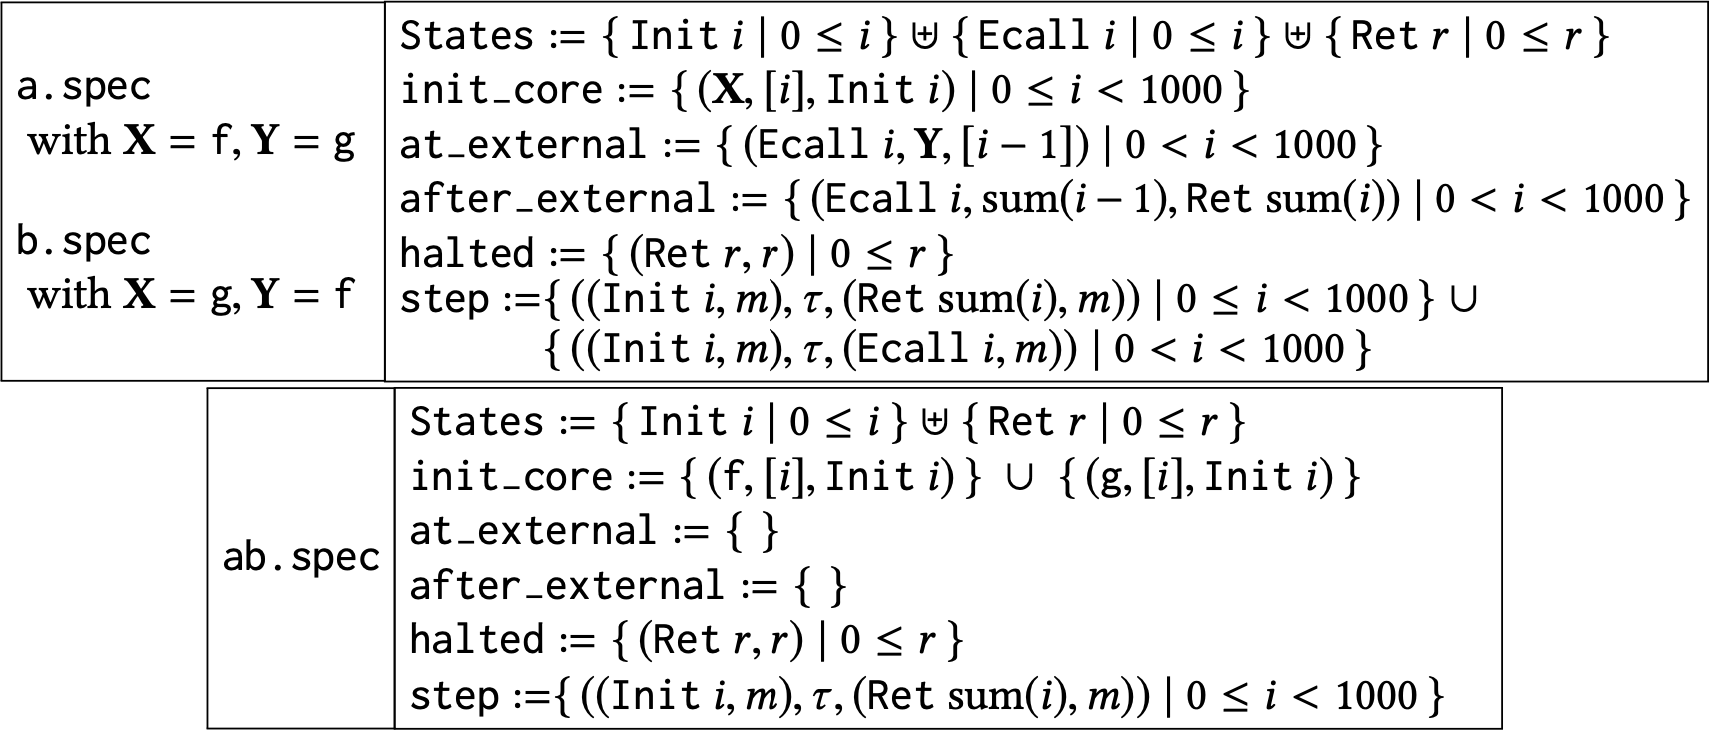
\includegraphics[width=1\linewidth]{images/mutsum2.png}
\end{minipage}
}}
\end{figure}

%% \begin{figure}[t]
%% \fbox{\begin{minipage}{1.15pc}\mbox{}\\[27.25mm]$\texttt{a.c}$\\[23.35mm]\mbox{}\end{minipage}}
%% \hspace*{-1.9mm}
%% \begin{minipage}{0.423\textwidth}
%% \begin{Verbatim}[frame=single]

%% static int memoized1[1000] = {0};
%% int f(int i)   {
%%   int sum;
%%   if (i == 0) return 0;
%%   sum = memoized1[i];
%%   if (sum == 0) {
%%     sum = g(i-1) + i;
%%     memoized1[i] = sum;
%%   }
%%   return sum;  
%% }


%% \end{Verbatim}
%% \end{minipage}
%% \hspace*{-2.0mm}
%% $\mbox{}~\mathlarger{\mathlarger{\mathlarger{\mathlarger{\mathlarger{\llink}}}}}~\mbox{}$
%% \hspace*{-2.2mm}
%% \fbox{\begin{minipage}{2.05pc}\mbox{}\\[26.21mm]$\texttt{b.asm}$\\[24.41mm]\mbox{}\end{minipage}}
%% \hspace*{-1.9mm}
%% \begin{minipage}{0.41\textwidth}
%% \begin{Verbatim}[frame=single]
%% // hand-optimized in assembly
%% static int memoized2[2] = {0,0};
%% int g(int i) {
%%   int sum;
%%   if (i == 0) return 0;
%%   if (i == memoized2[0]) {
%%     sum = memoized2[1];
%%   } else {
%%     sum = f(i-1) + i;
%%     memoized2[0] = i;
%%     memoized2[1] = sum;
%%   }
%%   return sum;
%% }
%% \end{Verbatim}
%% \end{minipage}
%% \\
%% \mbox{\fbox{\begin{minipage}{6.5pc}\mbox{}\\[2.13mm]$\texttt{a.spec}$ \\$\text{   with} ~ \textbf{X} = \texttt{f}, \textbf{Y} = \texttt{g}$\\[3.5mm]
%%       $\texttt{b.spec}$\\ $\text{   with} ~ \textbf{X} = \texttt{g}, \textbf{Y} = \texttt{f}$\\[0.33mm]\mbox{}\end{minipage}}
%% \hspace*{-1.9mm}
%% \fbox{\begin{minipage}{0.72\textwidth}
%%     $
%%   \texttt{States} := \setof{ \texttt{Init}\ i \ | \ 0 \leq i } \uplus \setof{ \texttt{Ecall} \ i\  |\  0 \leq i } \uplus \setof{ \texttt{Ret}\  r\  | \ 0 \leq r } \\
%%   \texttt{init\_core} := \setof{ (\textbf{X}, [i], \texttt{Init}\  i) \ |\  0 \leq i < 1000 } \\
%%   \texttt{at\_external} := \setof{ (\texttt{Ecall} \ i, \textbf{Y}, [i-1])\  |\  0 < i < 1000 } \\
%%   \texttt{after\_external} := \setof{ (\texttt{Ecall} \ i, \textrm{sum}(i-1), \texttt{Ret} \ \textrm{sum}(i))\  |\  0 < i < 1000 } \\
%%   \texttt{halted} := \setof{ (\texttt{Ret}\  r, r) \ |\  0 \leq r } \\
%%   \begin{aligned}
%%     \texttt{step} :=& \setof{ ((\texttt{Init} \ i, m), \tau, (\texttt{Ret}\  \textrm{sum}(i), m))\  |\  0 \leq i < 1000 } \ \cup \\[-1.5mm]
%%     &\setof{ ((\texttt{Init} \ i, m), \tau, (\texttt{Ecall}\  i, m))\  |\  0 < i < 1000 }\\[-1mm]
%%   \end{aligned}
%%   $
%% \end{minipage}}}
%% \\
%% \mbox{\fbox{\begin{minipage}{2.9pc}\mbox{}\\[8.73mm]$\texttt{ab.spec}$\\[6.93mm]\mbox{}\end{minipage}}
%% \hspace*{-1.9mm}
%% \fbox{\begin{minipage}{0.60\textwidth}
%%     $
%%   \texttt{States} := \setof{ \texttt{Init}\ i \ | \ 0 \leq i } \uplus \setof{ \texttt{Ret}\  r\  | \ 0 \leq r } \\
%%   \texttt{init\_core} := \setof{ (\texttt{f}, [i], \texttt{Init}\  i) } \ \cup \  \setof{ (\texttt{g}, [i], \texttt{Init}\  i) } \\
%%   \texttt{at\_external} := \setof{ } \\
%%   \texttt{after\_external} := \setof{ } \\
%%   \texttt{halted} := \setof{ (\texttt{Ret}\  r, r) \ |\  0 \leq r } \\
%%   \begin{aligned}
%%     \texttt{step} :=& \setof{ ((\texttt{Init} \ i, m), \tau, (\texttt{Ret}\  \textrm{sum}(i), m))\  |\  0 \leq i < 1000 }\\[-1mm]
%%   \end{aligned}
%%   $
%% \end{minipage}}}
%% \caption{The \code{mutual-sum} example}
%% \label{fig:modulelocal}
%% \end{figure}


\Cref{fig:modulelocal} shows a C module, \texttt{a.c}; a handwritten
assembly module, \texttt{b.asm} (presented in C syntax for
readability); their open specification modules, \texttt{a.spec} and
\texttt{b.spec}; and the combined closed specification module
\texttt{ab.spec}.  Both functions \texttt{f} in \texttt{a.c} and
\texttt{g} in \texttt{b.asm} mutually recursively compute the
summation from $0$ up to the given argument integer $i$ (denoted
$\mathrm{sum}(i)$), performing different memoization optimizations.
The function \code{f} memoizes the result of \code{f(i)} in the static
variable \code{memoized1[i]}, which is initialized with zero
representing invalid value.  The function call \code{f(i)} first reads
the memoized value, and returns it if it is valid; otherwise, it
calculates, memoizes, and returns \code{g(i-1)}, expected to be
$\mathrm{sum}(\code{i}-1)$, plus \code{i}.  On the other hand, the
function \code{g} memoizes only the result of the latest call
\code{g(i)} with the index \code{i}, where \code{memoized2[0]} =
\code{i} and \code{memoized2[1]} = \code{g(i)}.  The code of \texttt{g}
is self-explanatory under the assumption that the call \code{f(i-1)}
returns $\mathrm{sum}(\code{i}-1)$.

%% we have $\code{g(memoized[0])} = \code{memoized[1]}$.
%% The function \code{g(i)} is the same with
%% \code{f(i)}, except for memoization scheme, the callee of recursion,
%% and the language.

%% Our framework is flexible on the choice of languages to the degree that a module's (open)
%% specification can be represented as another module written in Coq's Gallina language.  Such
%% specification module facilitates modular verification of multi-language programs, as illustrated in
%% the example presented in \Cref{fig:modulelocal}.

%% Both of the function \code{f(i)} in the module \code{a.c} and \code{g(i)} in \code{b.asm} compute
%% $\textrm{sum}(\code{i})$, which is the summation from 1 to \code{i}, but with memoization and mutual
%% recursion on each other.\footnote{The module \code{b.asm} is written in hand-optimized assembly, but
%%   for presentational purposes we present it in C syntax.}  The module \code{a.c} memoizes the result
%% of \code{f(i)} in \code{memoized[i]}, which is initialized with zero representing invalid value.
%% The function \code{f(i)} first reads the memoized value, and returns it if valid; otherwise, it
%% calculates, memoizes, and then returns the summation of \code{g(i-1)}---which is expected to be
%% $sum(\code{i-1})$---and \code{i}.  On the other hand, \code{b.asm} memoizes only one result of
%% \code{g()}: we have $\code{g(memoized[0])} = \code{memoized[1]}$.  The function \code{g(i)} is the
%% same with \code{f(i)}, except for memoization scheme, the callee of recursion, and the language.


The open specification modules \texttt{a.spec} and \texttt{b.spec} are
the same except that the names of the internal and external functions
are swapped. This is natural because the two functions \code{f} and
\code{g} compute the same summation. The open specification
\texttt{a.spec} is an abstract, nondeterministic, version of the
function \texttt{f} in \texttt{a.c} including all the observable
behaviors of \texttt{f}.  It has three kinds of states,
$\code{Init}~i$, $\code{Ecall}~i$ and $\code{Ret}~r$, representing the
initial state with argument $i$, the call state executing
$\code{g}(i-1)$, and the halt state returning $r$, respectively. Then
\code{init\_core} starts with $\code{Init}~i$ when \texttt{f} is
invoked with argument $i$ if $0 \le i < 1000$, otherwise UB;
\code{at\_external} recognizes $\code{Ecall}~i$ as the state invoking
\texttt{g} with $i-1$; \code{after\_external} transitions
from $\code{Ecall}~i$ to $\code{Ret}~\mathrm{sum}(i)$ only
when the return value from the external call $\texttt{g}(i-1)$
is $\mathrm{sum}(i-1)$, otherwise UB, which
means that this module gives a conditional specification under the
assumption that $\texttt{g}(i)$ returns $\mathrm{sum}(i)$;
\code{halted} recognizes $\code{Ret}~r$ as the halted state returning
$r$; and finally $\code{step}$ transitions from $\code{Init}~i$ to
either $\code{Ret}~\mathrm{sum}(i)$ or $\code{Ecall}~i$
nondeterministically (without updating the memory), where the former
abstracts reading from memoization and the latter recursively
computing the sum. The same applies to \texttt{b.spec}.
Finally, the combined specification \code{ab.spec} does not make any
external function call and simply returns the summation.

Then, we perform our verification as follows.
First, we prove $\texttt{a.spec} \rusc_\rels \texttt{a.c}$
using memory injections with the following invariant:\\
%% \[
\mbox{}\hfill$\forall 0 \le i < 1000,~
\code{memoized1}[i] = 0 \lor \code{memoized1}[i] = \mathrm{sum}(i)~.$\hfill\mbox{}
%% \]
\\
Second, we prove $\texttt{b.spec} \rusc_\rels \texttt{b.asm}$
using memory injections with the following invariant:\\
%% \[
\mbox{}\hfill$
\exists 0 \le i < 1000,~
\code{memoized2}[0] = i \land \code{memoized2}[1] = \mathrm{sum}(i)~.
$\hfill\mbox{}
%% \]
\\
Finally, we prove $\texttt{ab.spec} \rusc_\rels \texttt{a.spec} \llink
\texttt{b.spec}$ using the memory identity.
\revision{Note that $\rels$ is the set containing open simulations with the three memory relations
  used in the above verification
  (\ie memory injections with the two invariants above and the memory identity).}

%% The module \code{ab.spec} represents a specification module for $\code{a.c} \llink \code{b.asm}$.
%% The specification essentially says \code{f(i)} and \code{g(i)} returns $sum(\code{i})$ if
%% $0 \le \code{i} < 1000$; otherwise, the behavior is undefined.  Note that the condition on \code{i}
%% comes from the fact that a bigger \code{i} causes buffer overrun at the access to \code{memoized[i]}
%% in \code{f(i)}.  Concretely, \code{ab.spec} has two kinds of states: \code{Init i} representing the
%% initial state with argument \code{i}, and \code{Ret res} representing the halted state with result
%% \code{res}; the module initializes a core with the initial state \code{Init i} when \code{f(i)} or
%% \code{g(i)} is invoked; an initial state \code{Init i} transitions to a return state \code{Ret
%%   $sum(\code{i})$} if $0 \le \code{i} < 1000$; and the module invokes no external function calls.

%% The verification of \code{a.c} and \code{b.asm} amounts to proving
%% $\beh{\texttt{ab.spec}} \supseteq \beh{\texttt{a.c} \llink \texttt{b.asm}}$, which comes from
%% linking the following verifications:
%% \[
%% \begin{array}{c}
%% \texttt{a.spec} \rusc_\rels \texttt{a.c}\quad
%% \texttt{b.spec} \rusc_\rels \texttt{b.asm}
%% \\
%% \texttt{ab.spec} \rusc_\rels \texttt{a.spec} \llink \texttt{b.spec}
%% \end{array}
%% \]
%% where $\rusc_\rels$ is the RUSC relation for a suitable set, $\rels$, of module relations, and
%% \code{a.spec} and \code{b.spec} are themselves (open) specification modules for \code{a.c} and
%% \code{b.asm}, respectively.  The specification module \code{a.spec} essentially says \code{f(i)},
%% provided that \code{i} is in a valid range, either $(i)$ returns $sum(\code{i})$; or $(ii)$ invokes
%% an external call \code{g(i-1)}, receives $sum(\code{i}-1)$ as a result, and then returns
%% $sum(\code{i})$.  To model the interaction with the external function call to \code{g(i-1)}, the
%% specification module has a state, \code{Ecall i}, that represents the call to \code{g(i-1)}.
%% Crucially, If the call does not return $sum(\code{i-1})$, the behavior is undefined.  The
%% specification module \code{b.spec} is the same with \code{a.spec}, except that \code{f} and \code{g}
%% are switched.

%% Verifications of $\texttt{a.spec} \rusc_\rels \texttt{a.c}$ and
%% $\texttt{b.spec} \rusc_\rels \texttt{b.asm}$ require module-local invariants, because the memoized
%% values in \code{memoized} should be private, as they exist only in the target, but they may be
%% changed during an external function call via mutual recursion.  As the module-local invariant, we
%% require that memoized values, if valid, are indeed correct.  On the other hand, verification of
%% $\texttt{ab.spec} \rusc_\rels \texttt{a.spec} \llink \texttt{b.spec}$ does not require module-local
%% invariants and any other complications from programming language semantics, but require reasoning
%% about multiple modules.

%% Specification module not only facilitates modular verification of multi-language programs, thereby
%% reducing the total verification cost, but also enables verification of handwritten assembly
%% functions whose correctness is axiomatized in \cc{}, reducing its trusted computing base (TCB).  See
%% \Cref{sec:utod-verification} for details.

{\revisioncmd
\subsection{Verification of \texttt{utod}}
\label{sec:overview-modulelocal:utod}

\verb|__compcert_i64_utod| is one of the \cc{}'s internal handwritten
assembly functions, which converts \verb|unsigned long| to
\verb|double| by utilizing architecture-specific instructions like
\verb|cvtsi2sdq|. \cc{} currently axiomatizes the behaviors of such runtime libraries as the following axiom.

\begin{figure}[t]
%% \makebox[\linewidth]{\makebox[1.1\linewidth]{
%% \begin{minipage}{1.1\linewidth}
%% 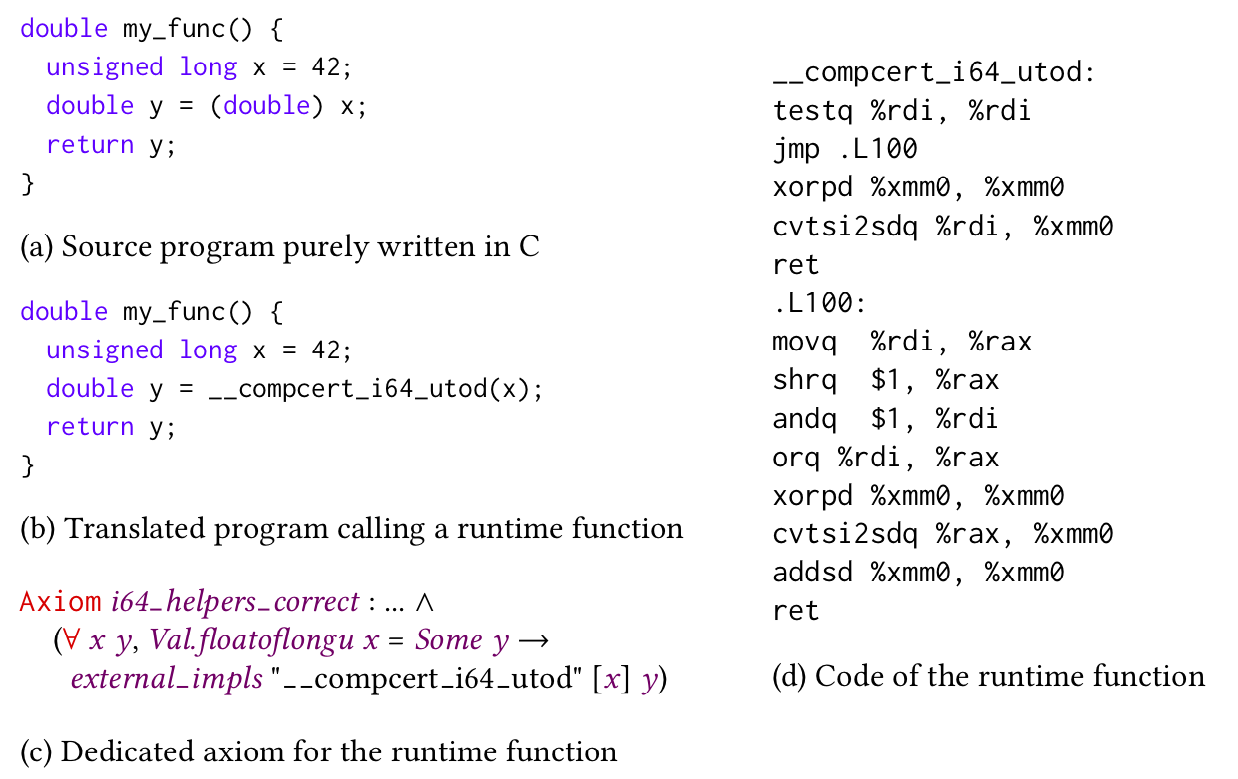
\includegraphics[width=1\linewidth]{images/utod.png}
%% \end{minipage}
%% }}
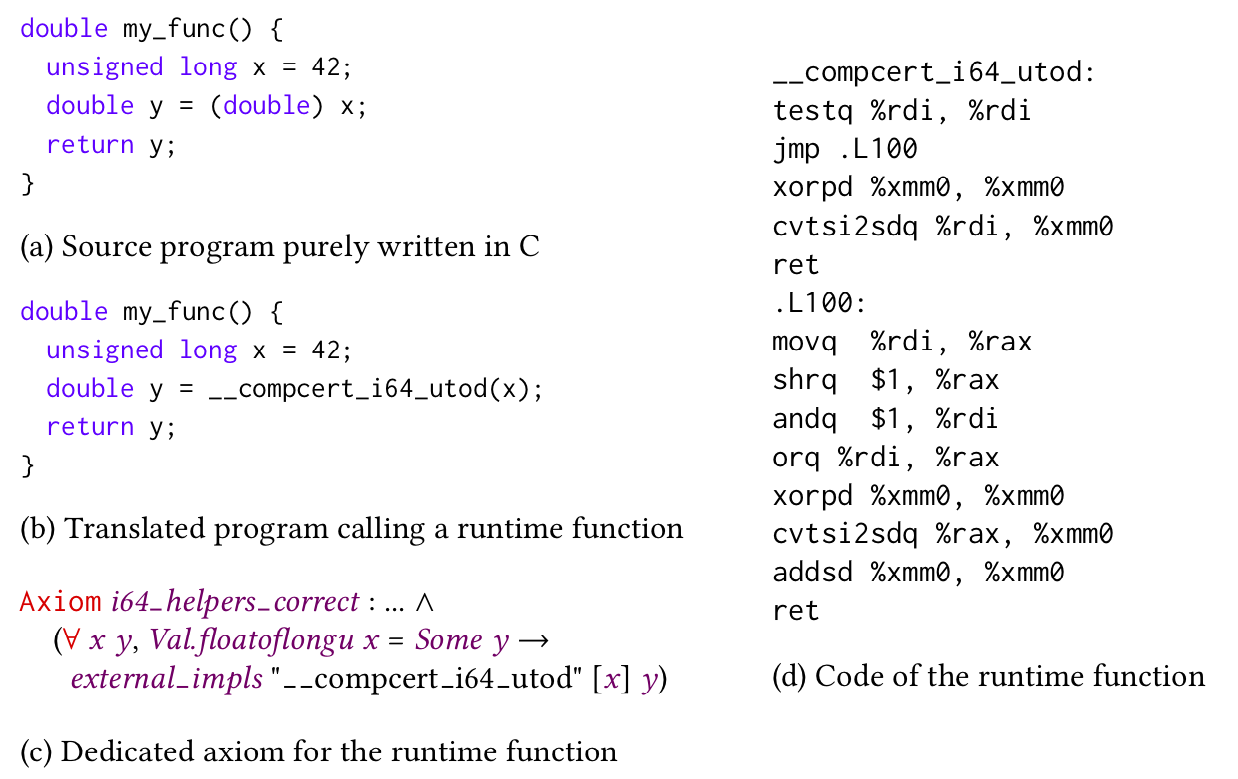
\includegraphics[width=1\linewidth]{images/utod.png}
\end{figure}

\[
\begin{minipage}{\textwidth}
\begin{coqdoccode}
\coqdocnoindent
\coqdockw{Axiom} \coqdoccst{i64\_helpers\_correct} : ... \ensuremath{\land}\coqdoceol
\coqdocindent{0.5em}
(\coqdockw{\ensuremath{\forall}} \coqdocvar{x} \coqdocvar{z}, \coqdocmod{Val}.\coqdoccst{floatoflongu} \coqdocvar{x} = \coqdocconstr{Some} \coqdocvar{z} \ensuremath{\rightarrow}
\coqdoccst{external\_implements} "\_\_compcert\_i64\_utod" \coqdoccst{sig\_l\_f} [\coqdocvar{x}] \coqdocvar{z})
\end{coqdoccode}
\end{minipage}
\]

We demonstrate that such axioms can be essentially removed in \ccm{} by proving the axiom for \verb|__compcert_i64_utod|.
We first turn the axiom for \verb|__compcert_i64_utod| into a specification module
and then establish an open simulation with memory injections between the assembly module containing \verb|__compcert_i64_utod| and the specification module.
}






%% \section{Background}
%% \label{sec:program:background}

%% \section{Problems}
%% \label{sec:program:problems}

%% \section{Solution}
%% \label{sec:program:solution}

\todo{put trimmed table from CompCertM}
